	\documentclass[10pt,oneside]{CBFT_book}
	% Algunos paquetes
	\usepackage{amssymb}
	\usepackage{amsmath}
	\usepackage{graphicx}
	\usepackage{libertine}
	\usepackage[bold-style=TeX]{unicode-math}
	\usepackage{lipsum}

	\usepackage{natbib}
	\setcitestyle{square}

	\usepackage{polyglossia}
	\setdefaultlanguage{spanish}
	



	\usepackage{CBFT.estilo} % Cargo la hoja de estilo

	% Tipografías
	% \setromanfont[Mapping=tex-text]{Linux Libertine O}
	% \setsansfont[Mapping=tex-text]{DejaVu Sans}
	% \setmonofont[Mapping=tex-text]{DejaVu Sans Mono}

	%===================================================================
	%	DOCUMENTO PROPIAMENTE DICHO
	%===================================================================

\begin{document}

% =================================================================================================
\chapter{Partículas idénticas}
% =================================================================================================

Más apropiado sería partículas indistinguibles. Si en algún punto del espacio se solapan las funciones de 
onda (interfieren) de dos partículas del mismo tipo cosa de que tengan misma masa, carga, etc. (dos 
electrones por ejemplo) no podemos distinguir cual es cual. Sean dos estados $\Ket{k'},\Ket{k''}$ con $k^{(i)}$ 
índice colectivo. En la zona de interferencia es 
\[
	\Ket{k'}_1 \otimes \Ket{k'}_2 \quad \text{o} \quad \Ket{k''}_1 \otimes \Ket{k''}_2
\]
donde ambos estados son ortogonales y los subíndices numéricos identifican a la partícula. 

\begin{figure}[htb]
	\begin{center}
	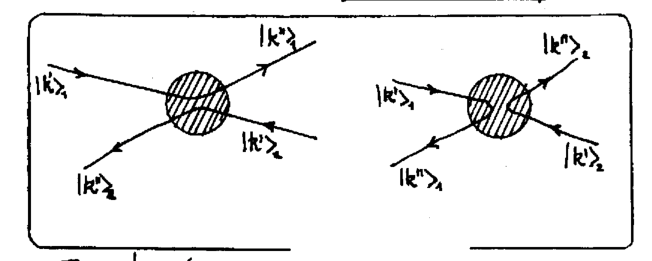
\includegraphics[width=0.9\textwidth]{images/teo2_29.pdf}
	\end{center}
	\caption{}
\end{figure} 
Entonces un estado general será
\[
	\Ket{K} = c_1 \Ket{k'}_1 \otimes \Ket{k''}_2 + c_2 \Ket{k''}_1 \otimes \Ket{k'}_2
\]
con $|c_1|^2 +|c_2|^2= 1$. 
Esta es la ``degeneración de intercambio''.

\subsection{Permutación}

Definimos este operador como 
\[
	P_{12}( \Ket{k'}_1\otimes \Ket{k''}_2 ) = \Ket{k''}_1\otimes \Ket{k'}_2
\]
\[
	P_{12} = P_{21} \qquad P_{12}^2 = \mathbb{1} \qquad P_{12}^\dagger = P_{12} \qquad 
	P_{12}P_{12}^\dagger = 1 \qquad \text{autovalores:} \; \pm 1
\]
Su función es la de intercambiar etiquetas, no el orden de las partículas.
Sean operadores $\hat{A}_1,\hat{A}_2$ que actúan sobre las partículas 1,2; es decir 
\[
	\hat{A}_1 \equiv \hat{A}_1\otimes\mathbb{1}_2, \qquad 
	\hat{A}_2 \equiv \mathbb{1}_1\otimes\hat{A}_2
\]
\[
	\hat{A}_1 \Ket{a'} \Ket{a''} = a' \Ket{a'} \Ket{a''} \qquad 
	\hat{A}_2 \Ket{a'} \Ket{a''} = a'' \Ket{a'} \Ket{a''} 
\]
\[
	P_{12}A_1P_{12}^{-1}P_{12}\Ket{a'} \Ket{a''} = P_{12} a' \Ket{a'}_1 \Ket{a''}_2 =
	a' \Ket{a''}_1 \Ket{a'}_2
\]
\[
	= P_{12}A_1P_{12}^{-1} \Ket{a''}_1 \Ket{a'}_2 = a' \Ket{a''}_1 \Ket{a'}_2
\]
\[
	= A_2 \Ket{a''}_1 \Ket{a'}_2 = a' \Ket{a''}_1 \Ket{a'}_2
\]
y
\[
	P_{12}\hat{A}_1P_{12}^{-1} = \hat{A}_2, \qquad P_{21} A_1 - A_2 P_{12} = 0
\]

Luego $\hat{A}$ es simétrico si $[\hat{P}_{12},\hat{A}_{12}]=0$. Sea $[\hat{P}_{12},\hat{H}]=0$ entonces es 
$P_{12}$ constante de movimiento y 
\[
	P_{12} \Ket{\alpha} = \pm \Ket{\alpha}
\]
Sea 
\[
	H = \frac{p_1^2}{2m_1} + \frac{p_2^2}{2m_2} + v(|x_1 - x_2|) + V_e(\vb{x}_1)+ V_e(\vb{x}_2)
\]
donde si las partículas son idénticas es $m_1=m_2\equiv m$ y defino dos estados
\[
	\Ket{k' k''}_s = \frac{1}{\sqrt{2}}\left( \Ket{k'}_1\Ket{k''}_2 + \Ket{k''}_1\Ket{k'}_2 \right) \qquad 
	\Ket{k' k''}_a = \frac{1}{\sqrt{2}}\left( \Ket{k'}_1\Ket{k''}_2 - \Ket{k''}_1\Ket{k'}_2 \right)
\]
con 
\[
	P_{12}\Ket{\phantom{k}}_s = + \Ket{\phantom{k}}_s \qquad \qquad 
	P_{12}\Ket{\phantom{k}}_a = - \Ket{\phantom{k}}_a
\]
Puedo introducir operadores de simetrización y antisimetrización 
\[
	\hat{S}_{12} \equiv \frac{1}{\sqrt{2}} \left( \mathbb{1} + \hat{P}_{12} \right)
\]
\[
	\hat{A}_{12} \equiv \frac{1}{\sqrt{2}} \left( \mathbb{1} - \hat{P}_{12} \right)
\]
que verifican 
\[
	S^2 = S, \quad  A^2= A, \quad SA=AS=0, \quad [S,A] = 0
\]
\[
	\hat{S}_{12} (c_1\Ket{k'}\Ket{k''} + c_2\Ket{k''}\Ket{k'} ) = \frac{1}{\sqrt{2}}(c_1+c_2)
	(\Ket{k'}\Ket{k''} + \Ket{k''}\Ket{k'} )
\]
es simétrico y 
\[
	\hat{A}_{12} (c_1\Ket{k'}\Ket{k''} + c_2\Ket{k''}\Ket{k'} ) = \frac{1}{\sqrt{2}}(c_1-c_2)
	(\Ket{k'}\Ket{k''} - \Ket{k''}\Ket{k'} )
\]
es antisimétrico.
En general se complica bastante con más de dos partículas 
\[
	P_{ij}(\Ket{k'}_1\Ket{k''}_2...\Ket{k^i}_i...\Ket{k^j}_j...) =
	(\Ket{k'}_1\Ket{k''}_2...\Ket{k^j}_i...\Ket{k^i}_j...)
\]
pués tenemos 
\[
	[P_{ij},P_{k\ell}] \neq 0 \quad \text{en general}
\]
Las permutaciones para tres partículas pueden descomponerse 
\[
	P_{123} = P_{12}P_{13} 
\]
\[
	P_{123}\Ket{k'}\Ket{k''}\Ket{k'''} = P_{12}\Ket{k'''}\Ket{k''}\Ket{k'} = \Ket{k''}\Ket{k'''}\Ket{k'}
\]

Con tres partículas hay $3!$ estados; uno totalmente simétrico $\Ket{\phantom{k}}_s$, uno totalmente antisimétrico 
$\Ket{\phantom{k}}_a$ y cuatro sin simetría definida.
En estados simétricos serán 
\begin{align*}
	\Ket{k'k''k'''}_{s/a} = \frac{1}{\sqrt{6}}&\left( \Ket{k'k''k'''} +  \Ket{k''k'''k'} + \Ket{k'''k'k''}\right. \\
	& \left. \pm \Ket{k''k'k'''} \pm \Ket{k'k'''k''} \pm \Ket{k'''k''k'} \right)
\end{align*}
donde el $\Ket{}_a$ tiene el signo $(-)$ en las permutaciones anticíclicas y el $(+)$ en las cíclicas.
Existe un determinante de Slater como método mnemotécnico de obtener los estados $\Ket{}_a$.
\[
	\Ket{ \Psi }_a = \frac{1}{3!}\begin{vmatrix} \; \Ket{k'} & \Ket{k''} & \Ket{k'''} \\  
	\; \Ket{k'} & \Ket{k''} & \Ket{k'''} \\ \; \Ket{k'} & \Ket{k''} & \Ket{k'''} \end{vmatrix}
\]
La obtención de estos estados corresponde a aplicar 
\[
	A_{123} = \frac{1}{\sqrt{3!}}\left( \mathbb{1} + P_{231} + P_{312} - P_{212} - P_{132} - P_{321} \right)
\]
\[
	( \mathbb{1} + P_{23}P_{21} + P_{31}P_{32} - P_{21}P_{23} - P_{13}P_{12} - P_{32}P_{31} )
\]
Si dos $k^{(i)}$ coinciden ya no hay estado antisimétrico posible.

\section{Postulado de simetrización}

Permitirá romper la degeneración de intercambio. 
Postulamos que toda partícula es de uno de dos tipos de acuerdo a su simetría 

\begin{center}
\begin{tabular}{|c|l|l|l|l|}
\multirow{2}{*}{Sistemas de N part. idénticas} & N & simetrica & BE & entero\\
& N & antisimetrica & FD & semientero
\end{tabular}
\end{center}

En la naturaleza no ocurren simetrías mixtas.

\subsection{Principio de exclusión de Pauli}

Para fermiones supongamos sistema de dos partículas idénticas 
\[
	\Ket{ \Psi }_a = \frac{1}{\sqrt{2}}( \Ket{k'}_1\Ket{k''}_2 - \Ket{k''}_1\Ket{k'}_2)
\]
y entonces si $k'=k''$ se tiene que 
\[
	\Ket{ \Psi }_a = 0.
\]

No es posible tener dos fermiones con iguales números cuánticos. Por el contrario los bosones sí pueden tener 
iguales números cuánticos.

\subsection{Sistema de dos electrones de spin $1/2$}

Sistema de dos electrones de spin $1/2$. Son fermiones. Sea que $[H,S]=0$  con $S = S_1 + S_2$. Se tendrá 
\[
	\Ket{\Psi}^{sist} = \Ket{\Psi}^{spa} \otimes \Ket{\Psi}^{spin}
\]
Como $\Ket{\Psi}^{sist}$ es simétrica tendremos 
\[
	P_{12} \Ket{\Psi}^{sist} = - \Ket{\Psi}^{sist} 
\]
\[
	P_{12} \Ket{\Psi}^{sist} = P_{12} \Ket{\Psi}^{spa} \otimes P_{12}\Ket{\Psi}^{spin} 
\]

Para dos electrones con spin $1/2$ se tiene $j_1+j_2$ entonces $ 0 \leq j \leq 1 $ de modo que $|m_1|\leq j_1$ y
$|m_2|\leq j_2$ entonces $0 \leq S \leq 1$ y $|m_{s_1}|\leq s_1$ y $|m_{s_2}|\leq s_1$.
\[
	\left.\begin{aligned}
	& \Ket{\uparrow \uparrow} \\
	& \Ket{\downarrow \downarrow } \\
	& \frac{1}{\sqrt{2}}( \Ket{ \uparrow\downarrow }+\Ket{ \downarrow\uparrow} )
	\end{aligned}
	\right\} \; \text{triplete} \; s=1 \qquad \text{Estados simétricos}
\]
\[
	\left.\begin{aligned}
	\frac{1}{\sqrt{2}}( \Ket{\uparrow\downarrow} - \Ket{\downarrow\uparrow} )
	\end{aligned}
	\right\} \; \text{singlete} \; s=0 \qquad \text{Estados antisimétricos}
\]
Entonces
\begin{gather*}
	\begin{aligned}
	s=0 \qquad \Rightarrow \; &\Ket{\Psi}^{spa} \text{es simétrica} \\
	s=1 \qquad \Rightarrow \; &\Ket{\Psi}^{spa} \text{es antisimétrica}
	\end{aligned}	
\end{gather*}	

Vistos desde el CM de los electrones
\[
	P_{12} = \Pi
\]
y entonces
\[
	P_{12}\Ket{n\ell m} = (-1)^\ell \Ket{n\ell m}
\]
\[
	\ell \;\text{par} \; \rightarrow \Ket{\Psi}^{spa} = P_{12} \Ket{\Psi}^{spa} \qquad 
	\ell \;\text{impar} \; \rightarrow -\Ket{\Psi}^{spa} = P_{12} \Ket{\Psi}^{spa}
\]
Necesitaré $\ell$ par con $s=0$ entonces $\ell+s=j$ par. En cambio, si $\ell$ impar con $s=1$ entonces 
$\ell+s=j$ par. Dos electrones sólo se acoplan a momento total $j$ par.

Sean los siguientes estados 
\[
	\Ket{ \Psi }_{sa} = \frac{1}{\sqrt{2}}( \Ket{k'}\Ket{k''} \pm \Ket{k''}\Ket{k'})
\]
\[
	\Ket{ \Psi_F }_{sa} = \frac{1}{\sqrt{2}}( \Ket{a'}\Ket{a''} \pm \Ket{a''}\Ket{a'})
\]
y la probabilidad será
\[
	\text{Prob}\; = |_{sa}\Braket{\Psi|\Psi}_{sa}|^2 = 
	\left|\frac{1}{2}(_1\Bra{a'}_2\Bra{a''} \pm _1\Bra{a''}_2\Bra{a'})(\Ket{k'}_1\Ket{k''}_2 \pm 
	\Ket{k''}_1\Ket{k'}_2)\right|^2 =
\]
\[
	= \frac{1}{4}\left| \Bra{a'}\Bra{a''}\Ket{k'}\Ket{k''} \pm \Bra{a''}\Bra{a'}\Ket{k'}\Ket{k''} 
	\pm \Bra{a'}\Bra{a''}\Ket{k''}\Ket{k'} \pm \Bra{a''}\Bra{a'}\Ket{k''}_1\Ket{k'} \right|^2
\]
\[
	= \frac{1}{4}\left| 2\Braket{a'|k'}\Braket{a''|k''} \pm 2\Braket{a''|k'}\Braket{a'|k''}\right|^2
\]
\[
	= \left| \underbrace{\Braket{a'|k'}\Braket{a''|k''}}_{\text{término directo}} \pm 
	\underbrace{\Braket{a''|k'}\Braket{a'|k''}}_\text{término de intercambio}\right|^2
\]
\begin{multline*}
	\text{Prob}\; = |_{sa}\Braket{\Psi|\Psi}_{sa}|^2 = \left| \Braket{a'|k'}\Braket{a''|k''} \right|^2 + 
	\left|\Braket{a''|k'}\Braket{a'|k''}\right|^2 \\
	\pm 2\mathcal{Re}\left(\underbrace{ \Braket{a'|k'}\Braket{a'|k''}^*\Braket{a''|k''}\Braket{a''|k'}^* 
	}_\text{Interferencia}\right)
\end{multline*}

Vemos que aparece una interferencia que será importante solamente si hay solapamiento. En el caso de no 
solaparse o con partículas clásicas solo el primer término es de importancia.

\section{El átomo de helio}


\begin{figure}[htb]
	\begin{center}
	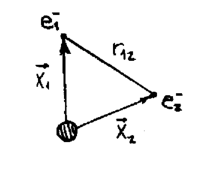
\includegraphics[width=0.4\textwidth]{images/teo2_30.pdf}
	\end{center}
	\caption{}
\end{figure} 
\[
	H = \frac{p_1}{2m} + \frac{p_2}{2m} - \frac{2e^2}{r_1} -  \frac{2e^2}{r_2} + \frac{e^2}{r_{12}}
\]
y si el último término es $\sim 0$ decimos que en ese caso $H$ está desacoplado 
\[
	\Psi = \Psi_1 \otimes \Psi_2
\]
\[
	[\vb{H},\vb{S}] = 0 \qquad \vb{S} = \vb{S}_1 + \vb{S}_2 = \begin{cases} 0 \\ 1 \end{cases}
\]
S es constante de movimiento y para la $\Ket{\psi_{spin}}$ se tiene 
\[
	S=0 \qquad \frac{1}{\sqrt{2}}( \Ket{ \uparrow\downarrow }-\Ket{ \downarrow\uparrow}) \quad \text{singlete}
\]
\[
	S=1 \qquad \begin{aligned}
	& \Ket{\uparrow \uparrow} \\
	& \Ket{\downarrow \downarrow } \\
	& \frac{1}{\sqrt{2}}( \Ket{ \uparrow\downarrow }+\Ket{ \downarrow\uparrow} )
	\end{aligned} \quad \text{triplete}
\]
Sea $ e^-_1 \Ket{100}$ y $e^-_2 \Ket{n\ell m}$
\[
	\Ket{\Psi}_{He} = \frac{1}{\sqrt{2}}\left(  \Ket{100}\Ket{n\ell m} \pm  \Ket{n\ell m}\Ket{100}
	\right) \Ket{\Psi_{spin}}
\]
de modo que con $S=0$ será
\[
	\Ket{\Psi}_{He} = \frac{1}{\sqrt{2}}\left( \Ket{100}\Ket{n\ell m} + \Ket{n\ell m}\Ket{100}\right) 
	\frac{1}{\sqrt{2}}( \Ket{ \uparrow\downarrow }-\Ket{ \downarrow\uparrow})
\]
y en cambio con $S=1$
\[
	\Ket{\Psi}_{He} = \frac{1}{\sqrt{2}}\left(  \Ket{100}\Ket{n\ell m} - \Ket{n\ell m}\Ket{100}\right) 
			\begin{cases}
	                   \Ket{\uparrow \uparrow} \\
			   \Ket{\downarrow \downarrow } \\
			   \frac{1}{\sqrt{2}}( \Ket{ \uparrow\downarrow }+\Ket{ \downarrow\uparrow} )
	                  \end{cases}
\]

Podemos pensar en teoria de perturbaciones ahora y calcular 
\[
	E_{He} = E_{100} + E_{n\ell m} + \Delta E
\]
donde 
\[
	\Delta E = \Braket{\Psi|\frac{e}{r_{12}}|\Psi}
\]
y el término en el {\it sandwich} lo considero una perturbación.
\[
	\Delta E = \Bra{\Psi^{spin}}^\dagger \frac{1}{2}\left(\Bra{100}\Bra{n\ell m} \pm \Bra{n\ell m}\Bra{100}
	\right) \frac{e}{r_{12}} \left(\Ket{100}\Ket{n\ell m} \pm \Ket{n\ell m}\Ket{100}\right)\Ket{\Psi^{spin}}
\]
\[
	\Delta E = \Bra{100}\Bra{n\ell m}\frac{e}{r_{12}}\Ket{100}\Ket{n\ell m} \pm  
	\Bra{n\ell m}\Bra{100}\frac{e}{r_{12}}\Ket{100}\Ket{n\ell m}
\]
que se puede escribir más resumidamente como
\[
	\Delta E = I \pm J
\]

\begin{figure}[htb]
	\begin{center}
	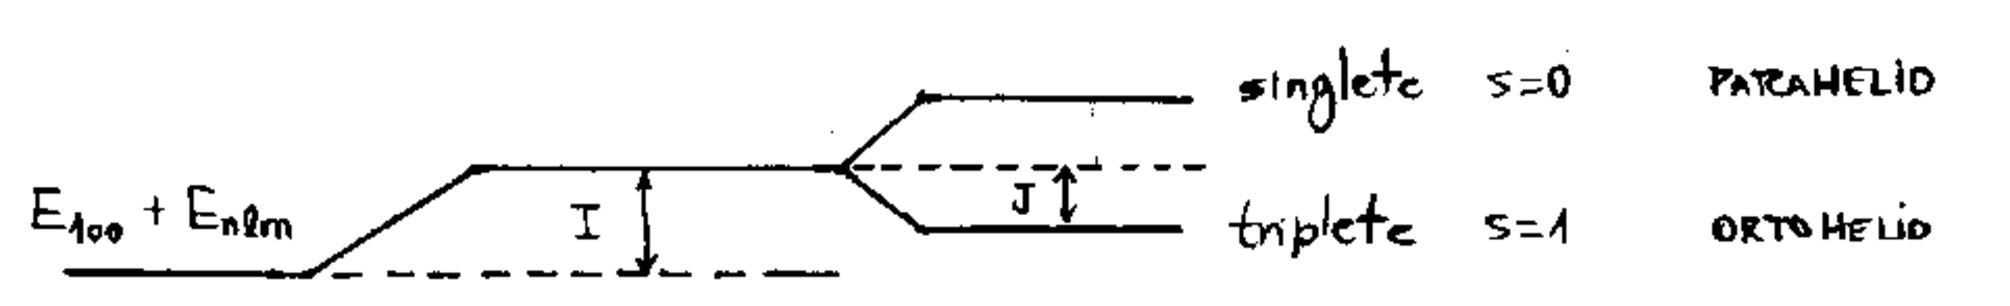
\includegraphics[width=1.0\textwidth]{images/teo2_15.pdf}
	\end{center}
	\caption{}
\end{figure} 

Esta separación de los niveles en $\pm J$ se debe al carácter de fermión de las partículas.



% \bibliographystyle{CBFT-apa-good}	% (uses file "apa-good.bst")
% \bibliography{CBFT.Referencias} % La base de datos bibliográfica

\end{document}
